%# -*- coding: utf-8 -*-
%!TEX encoding = UTF-8 Unicode
%!TEX TS-program = xelatex
% vim:ts=4:sw=4
%
% 以上设定默认使用 XeLaTex 编译,并指定 Unicode 编码,供 TeXShop 自动识别

% Author: Yunhui Fu <yhfudev@gmail.com>
% License: Creative Commons (CC BY 4.0)

\section{\cnt{Linear Decoders with Autoencoders}{自编码线性解码器}{}}

\subsection{\cnt{Linear Decoders}{线性解码器}{}}

\subsubsection{\cnt{Sparse Autoencoder Recap}{稀疏自编码重述}{}} \label{chp:sparseautoencrecap}

\cnt{In the sparse autoencoder, we had 3 layers of neurons: an input layer, a hidden layer and an output layer. In our previous description of autoencoders (and of neural networks), every neuron in the neural network used the same activation function. In these notes, we describe a modified version of the autoencoder in which some of the neurons use a different activation function. This will result in a model that is sometimes simpler to apply, and can also be more robust to variations in the parameters.}
    {稀疏自编码器包含3层神经元,分别是输入层,隐含层以及输出层。 从前面(神经网络)自编码器描述可知,位于神经网络中的神经元都采用相同的激励函数。 在注解中,我们修改了自编码器定义,使得某些神经元采用不同的激励函数。这样得到的模型更容易应用,而且模型对参数的变化也更为鲁棒。 }
    {}

\cnt{Recall that each neuron (in the output layer) computed the following:}
    {回想一下,输出层神经元计算公式如下:}
    {}
\begin{align} z^{(3)} &= W^{(2)} a^{(2)} + b^{(2)} \\ a^{(3)} &= f(z^{(3)}) \end{align}

\cnt{where $a^{(3)}$ is the output. In the autoencoder, $a^{(3)}$ is our approximate reconstruction of the input $x = a^{(1)}$.}
    {其中 $a^{(3)}$ 是输出. 在自编码器中, $a^{(3)}$ 近似重构了输入 $x = a^{(1)}$。 }
    {}

\cnt{Because we used a sigmoid activation function for $f(z^{(3)})$, we needed to constrain or scale the inputs to be in the range $[0,1]$, since the sigmoid function outputs numbers in the range $[0,1]$. While some datasets like MNIST fit well with this scaling of the output, this can sometimes be awkward to satisfy. For example, if one uses PCA whitening, the input is no longer constrained to $[0,1]$ and it's not clear what the best way is to scale the data to ensure it fits into the constrained range.}
    {S 型激励函数输出范围是 $[0,1]$,当 $f(z^{(3)})$ 采用该激励函数时,就要对输入限制或缩放,使其位于 $[0,1]$ 范围中。一些数据集,比如 MNIST,能方便将输出缩放到 $[0,1]$ 中,但是很难满足对输入值的要求。比如, PCA 白化处理的输入并不满足 $[0,1]$ 范围要求,也不清楚是否有最好的办法可以将数据缩放到特定范围中。}
    {}


\subsubsection{\cnt{Linear Decoder}{线性解码器}{}}

\cnt{One easy fix for this problem is to set $a^{(3)} = z^{(3)}$. Formally, this is achieved by having the output nodes use an activation function that's the identity function $f(z) = z$, so that $a^{(3)} = f(z^{(3)}) = z^{(3)}$. This particular activation function $f(\cdot)$ is called the linear activation function (though perhaps ``identity activation function" would have been a better name). Note however that in the hidden layer of the network, we still use a sigmoid (or tanh) activation function, so that the hidden unit activations are given by (say) $a^{(2)} = \sigma(W^{(1)}x + b^{(1)})$, where $\sigma(\cdot)$ is the sigmoid function, x is the input, and $W^{(1)}$ and $b^{(1)}$ are the weight and bias terms for the hidden units. It is only in the output layer that we use the linear activation function.}
    {设定 $a^{(3)} = z^{(3)}$ 可以很简单的解决上述问题。从形式上来看,就是输出端使用恒等函数 $f(z) = z$ 作为激励函数,于是有 $a^{(3)} = f(z^{(3)}) = z^{(3)}$。我们称该特殊的激励函数为 线性激励函数 (称为恒等激励函数可能更好些)。
    需要注意,神经网络中隐含层的神经元依然使用S型(或者$\tanh$)激励函数。这样隐含单元的激励公式为 $a^{(2)} = \sigma(W^{(1)}x + b^{(1)})$,其中 $\sigma(\cdot)$ 是 S 型函数, $x$ 是输入, $W^{(1)}$ 和 $b^{(1)}$ 分别是隐单元的权重和偏差项。我们仅在输出层中使用线性激励函数。

一个 S 型或 $\tanh$ 隐含层以及线性输出层构成的自编码器,我们称为线性解码器。}
    {}

\cnt{An autoencoder in this configuration--with a sigmoid (or tanh) hidden layer and a linear output layer--is called a linear decoder. In this model, we have $\hat{x} = a^{(3)} = z^{(3)} = W^{(2)}a + b^{(2)}$. Because the output $\hat{x}$ is a now linear function of the hidden unit activations, by varying $W^{(2)}$, each output unit $a^{(3)}$ can be made to produce values greater than 1 or less than 0 as well. This allows us to train the sparse autoencoder real-valued inputs without needing to pre-scale every example to a specific range.}
    {在这个线性解码器模型中,$\hat{x} = a^{(3)} = z^{(3)} = W^{(2)}a + b^{(2)}$。因为输出 $\hat{x}$ 是隐单元激励输出的线性函数,改变 $W^{(2)}$ ,可以使输出值 $a^{(3)}$ 大于 1 或者小于 0。这使得我们可以用实值输入来训练稀疏自编码器,避免预先缩放样本到给定范围。}
    {}

\cnt{Since we have changed the activation function of the output units, the gradients of the output units also change. Recall that for each output unit, we had set set the error terms as follows:}
    {随着输出单元的激励函数的改变,这个输出单元梯度也相应变化。回顾之前每一个输出单元误差项定义为: }
    {}
    \begin{align} \delta_i^{(3)} = \frac{\partial}{\partial z_i} \;\; \frac{1}{2} \left\|y - \hat{x}\right\|^2 = - (y_i - \hat{x}_i) \cdot f'(z_i^{(3)}) \end{align} 
\cnt{where $y = x$ is the desired output, $\hat{x}$ is the output of our autoencoder, and $f(\cdot)$ is our activation function. Because in the output layer we now have $f(z) = z$, that implies $f'(z) = 1$ and thus the above now simplifies to:}
    {其中 $y = x$ 是所期望的输出, $\hat{x}$ 是自编码器的输出, $f(\cdot)$ 是激励函数.因为在输出层激励函数为 $f(z) = z$, 这样 $f'(z) = 1$,所以上述公式可以简化为 }
    {}


    \begin{align} \delta_i^{(3)} = - (y_i - \hat{x}_i) \end{align} 

\cnt{Of course, when using backpropagation to compute the error terms for the hidden layer:}
    {当然,若使用反向传播算法来计算隐含层的误差项时: }
    {}


    \begin{align} \delta^{(2)} &= \left( (W^{(2)})^T\delta^{(3)}\right) \bullet f'(z^{(2)}) \end{align} 

\cnt{Because the hidden layer is using a sigmoid (or $\tanh$) activation $f$, in the equation above $f'(\cdot)$ should still be the derivative of the sigmoid (or $\tanh$) function.}
    {因为隐含层采用一个 S 型(或 $\tanh$)的激励函数 $f$, 在上述公式中,$f'(\cdot)$ 依然是 S 型(或 $\tanh$)函数的导数。 }
    {}



\subsection{\cnt{Exercise:Learning color features with Sparse Autoencoders}{练习:用线性解码器学习颜色特性}{}} \label{chp:execcolorfeaturesparseautoenc}

In this exercise, you will implement a linear decoder (\ref{chp:sparseautoencrecap}, a sparse autoencoder whose output layer uses a linear activation function). You will then apply it to learn features on color images from the STL-10 dataset. These features will be used in an later exercise on convolution and pooling for classifying STL-10 images.

In the file \href{http://ufldl.stanford.edu/wiki/resources/linear_decoder_exercise.zip}{linear\_decoder\_exercise.zip} we have provided some starter code. You should write your code at the places indicated ``YOUR CODE HERE" in the files.

For this exercise, you will need to copy and modify \texttt{sparseAutoencoderCost.m} from the sparse autoencoder exercise(\ref{chp:execsparseautoenc}).

\subsubsection{\cnt{Dependencies}{}{}}

You will need:

    \texttt{sparseAutoencoderCost.m} (and related functions) from Exercise:Sparse Autoencoder(\ref{chp:execsparseautoenc})

The following additional file is also required for this exercise:

    \href{http://ufldl.stanford.edu/wiki/resources/stl10_patches_100k.zip}{Sampled $8 \times 8$ patches from the STL-10 dataset (stl10\_patches\_100k.zip)}

If you have not completed the exercise listed above, we strongly suggest you complete it first.


\subsubsection{\cnt{Learning from color image patches}{}{}}

In all the exercises so far, you have been working only with grayscale images. In this exercise, you will get to work with RGB color images for the first time.

Conveniently, the fact that an image has three color channels (RGB), rather than a single gray channel, presents little difficulty for the sparse autoencoder. You can just combine the intensities from all the color channels for the pixels into one long vector, as if you were working with a grayscale image with $3 \times$ the number of pixels as the original image.

\subsubsection{\cnt{Step 0: Initialization}{}{}}


In this step, we initialize some parameters used in the exercise (see starter code for details).

\subsubsection{\cnt{Step 1: Modify your sparse autoencoder to use a linear decoder}{}{}}


Copy \texttt{sparseAutoencoderCost.m} to the directory for this exercise and rename it to \texttt{sparseAutoencoderLinearCost.m}. Rename the function sparseAutoencoderCost in the file to sparseAutoencoderLinearCost, and modify it to use a linear decoder((\ref{chp:sparseautoencrecap})). In particular, you should change the cost and gradients returned to reflect the change from a sigmoid to a linear decoder. After making this change, check your gradients to ensure that they are correct.

\subsubsection{\cnt{Step 2: Learn features on small patches}{}{}}


You will now use your sparse autoencoder to learn features on a set of 100,000 small $8 \times 8$ patches sampled from the larger $96 \times 96$ STL-10 images (The \href{http://www.stanford.edu/~acoates//stl10/}{STL-10 dataset} comprises 5000 training and 8000 test examples, with each example being a $96 \times 96$ labelled color image belonging to one of ten classes: airplane, bird, car, cat, deer, dog, horse, monkey, ship, truck.)

The code provided in this step trains your sparse autoencoder for 400 iterations with the default parameters initialized in step 0. This should take around 45 minutes. Your sparse autoencoder should learn features which when visualized, look like edges and ``opponent colors," as in the figure below.

\begin{figure}[ht] \centering
  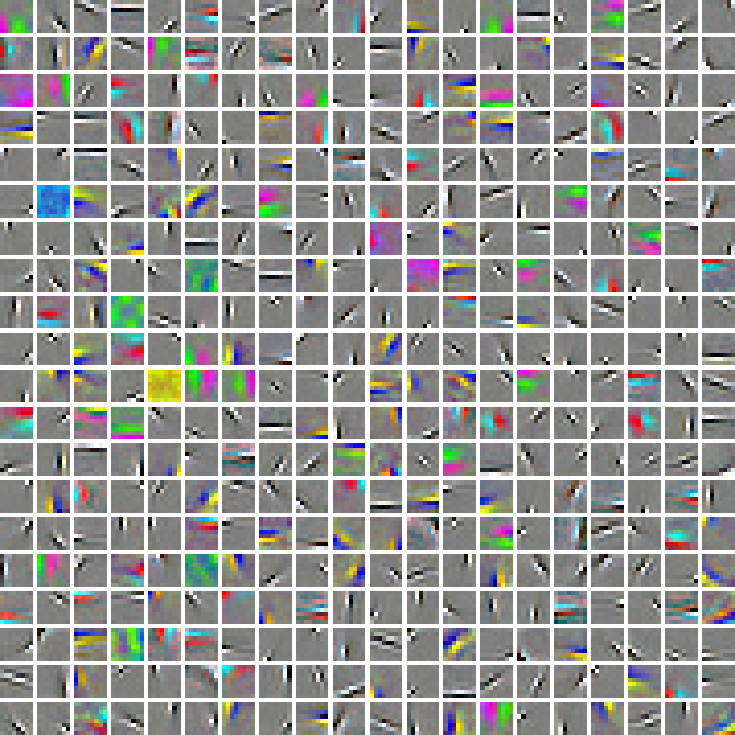
\includegraphics[width=0.5\textwidth]{figures/CNN_Features_Good.png}
  %\caption{}\label{fig:step1}
\end{figure}


\cnt{If your parameters are improperly tuned (the default parameters should work), or if your implementation of the autoencoder is buggy, you might instead get images that look like one of the following: }
    {}
    {}

\begin{figure}[ht] \centering
  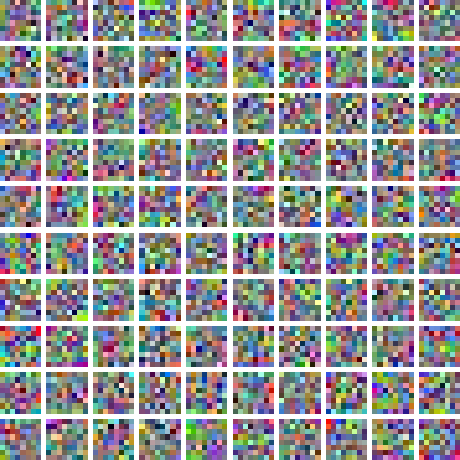
\includegraphics[width=0.5\textwidth]{figures/Cnn_Features_Bad1.png}
  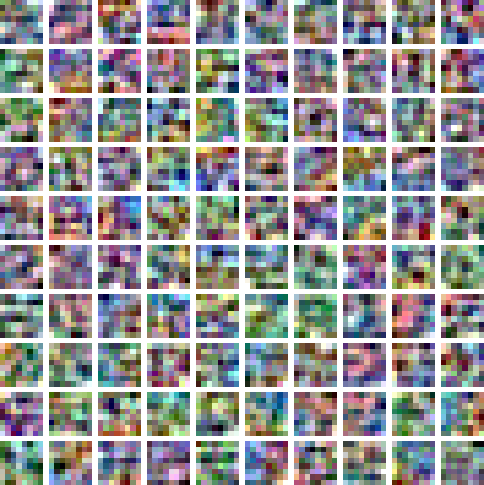
\includegraphics[width=0.5\textwidth]{figures/Cnn_Features_Bad2.png}
  %\caption{}\label{fig:step1}
\end{figure}


\cnt{The learned features will be saved to \texttt{STL10Features.mat}, which will be used in the later exercise on convolution and pooling(\ref{chp:execconvpool}). }
    {}
    {}

